% !TEX root = ../main.tex
\section{Theoretical Framework}
\label{sec:theory}
\subsection{Mixed logit}
\label{sec:mxl}
We start by introducing the mixed logit model in detail.
This is the model of interest for this thesis.
The mixwd logit can be derived from various behaviour specifications \citep{Train2009}.
We will show the derivation from a random coefficient discrete choice model.

In the model we assume that individual $i$, where $i = 1,\ldots,N$, makes a choice $j$ between $J$ alternatives and one outside good ($j=0$).
We model the latent utility $u_{ij}\in\mathbb{R}$ of individual $i$ for choice $j$ as
\begin{equation}
\label{eq:mxllatentutil}
    u_{ij} = \bm{x}_{ij}^\prime \bm{\beta}_{i} + \varepsilon_{ij},
\end{equation}
where $\bm{x}_{ij} \in \mathbb{R}^K$ denotes the column vector with observed exogenous variables for individual $i$, choice $j$.
Furthermore, $\bm{\beta}_{i}\in \mathcal{B} \subset \mathbb{R}^K$ denotes the unobserved column vector of individual-specific random coefficients, for individual $i$. 
Here, $\mathcal{B}$ denotes the support of the random coefficients.
When the random coefficients have finite support some speak of a latent class model, specifically the latent class multinomial logit model \citep{Train2009}.
In this model the elements of the support are often called ``types'', refering to the different types of individuals in the population.
The random coefficient vectors are independent and identically distributed (i.i.d.) draws from a cumulative distribution function $F_0$.\footnote{This means that for each individual $i$, the random coefficient vector $\bm{\beta}_{i}$ as a whole is jointly distributed as $F_0$. This does not mean that each element of a random coefficient vector is marginally distributed as $F_0$.}
The distribution function is not observed.
Next, $\varepsilon_{ij}\in \mathbb{R}$ denotes the unobserved idiosyncratic error term for individual $i$, choice $j$. 
The error terms are i.i.d. draws from a type I extreme value distribution.
Also, we assume strict exogeneity of the observed variables and independence of the unobserved components.
That is, $\mathbb{E}[\varepsilon_{ij}\mid \bm{x}_{i1}, \ldots,\bm{x}_{iJ}] = 0$ and $\bm{\beta}_i \perp \varepsilon_{ij}$ for all $i,j$.
At last, for $j=0$ (the outside good) we impose $u_{i0} = \varepsilon_{i0}$.

Let $y_{ij} \in \{0,1\}$ denote the indicator of the event that individual $i$ chooses the $j$th alternative. 
We assume individuals maximize utility. Then this implies
\begin{equation}
\label{eq:mxlydef}
    y_{ij} = \mathds{1}\{u_{ij} > u_{ik}, \text{ for all } j \neq k\} = \prod_{\substack{k=1; \\ k\neq j}}^{J}\mathds{1}\{u_{ij} > u_{ik}\}.
\end{equation}

As a researcher, the goal is often to estimate $F_0$ by $\hat{F}_0$, and possibly to conduct inference on this.
Sometimes the researcher is only interested in a parameter $\bm{\eta}$ that is specified by a (possibly vector-valued) functional $T$ of $F_0$, i.e. $\bm{\eta} = T(F_0)$.
A common estimator for $\bm{\eta}$ is the plug-in estimator $\hat{\bm{\eta}}$ defined by $\hat{\bm{\eta}} = T(\hat{F}_0)$ \citep[see][chap.~23]{vanderVaart1998}.
An example of such a parameter that is specified by a functional of $F_0$ is the population mean $\bm{\mu} = \mathbb{E}[\bm{\beta}]$.\footnote{Technically, we should specify that $\bm{\beta}\overset{\mathrm{d}}{=}\bm{\beta}_i$.}\footnote{To see that $\mu$ is indeed a parameter specified by a functional we notice that $\mu = T(F_0)$, where the functional $T: \mathcal{F} \to \mathbb{R}$ maps the distribution to the real line continuously via the integration $T(F) = \int_{\mathcal{X}_F} x \, \mathrm{d}F(x)$, where $\mathcal{F}$ denotes the space of all distribution functions and $\mathcal{X}_F$ denotes the support of $x$ distributed by $F$.}

A useful object of interest for estimation is the probability that $y_{ij} = 1$ conditional on $\bm{x}_i$, where we denote $\bm{x}_i = (\bm{x}_{i1}^\prime,\ldots,\bm{x}_{iJ}^\prime)$ as the stacked row vector of the exogenous variables for individual $i$.
The usefulness will become clear in \Cref{sec:FKRBestimator}.
Define
\begin{equation}
\label{eq:mxlgdef}
    g_j(\bm{x}_{i},\bm{\beta}_{i}) \coloneq \mathbb{P}(y_{ij} = 1 \mid \bm{x}_i, \bm{\beta}_i).
\end{equation}
We can derive an analytical expression \citep[see][chap.~3]{Maddala1983} in the form of
\begin{equation}
\label{eq:mxlganalytical}
    g_j(\bm{x}_{i},\bm{\beta}_{i}) = \frac{\exp{(\bm{x}_{ij}^\prime \bm{\beta}_i)}}{1 + \sum_{k=1}^{J}\exp{(\bm{x}_{ik}^\prime \bm{\beta}_i)}}.
\end{equation}
The only difference with \citet{Maddala1983} is that $\bm{\beta}_i$ is stochastic in our model. 
However, since we are also conditioning on $\bm{\beta}_i$, the derivation remains the same.
It then follows that
\begin{equation}
\label{eq:mxlcondprob}
    \mathbb{P}(y_{ij} = 1 \mid \bm{x}_{i}) = \int_{\mathcal{B}} g_j(\bm{x}_{i}, \bm{\beta}) \, \mathrm{d}F_{0}(\bm{\beta}).
\end{equation}

\subsection{FKRB Estimator}
\label{sec:FKRBestimator}
A commonly used estimator for the mixed logit is the estimator proposed by \citet{FoxKimRyanBajari2011}, which is hereafter referred to as the FKRB estimator.
They approximate the distribution of random coefficients by a finite mixture over fixed support points.
We then only need to find the probability mass at each support point to estimate $F_0$.
They rewrite \cref{eq:mxlcondprob} such that the probability masses enter the equation linearly.
Then they show that these can be consistently estimated by means of (constrained) least squares.

\subsubsection{Derivation}
\label{sec:FKRBderivation}
For completeness, we first show the derivation of the estimator. 
For some $R \in \mathbb{N}_+$, let $\tilde{\mathcal{B}} = \{\bm{\beta}^{(1)}, \bm{\beta}^{(2)}, \ldots, \bm{\beta}^{(R)}\}$.
Both $R$ and $\bm{\beta}^{(r)}$ should not be parameters of the model; they should be prespecified.\footnote{There exists an extension of the estimator where these do not have to be prespecified, but depend on the sample size $N$. This is dicussed in \cref{sec:nonparametricFKRB}.} 
We let $\theta_r$ denote the value of the probability mass function of $\bm{\beta}_{i}$ at $\bm{\beta}^{(r)}$, i.e. $\theta_r = \mathbb{P}(\bm{\beta}_{i} = \bm{\beta}^{(r)})$.
Then under the assumption $\tilde{\mathcal{B}} = \mathcal{B}$ we have that \cref{eq:mxlcondprob} boils down to
\begin{equation}
\label{eq:FKRBpij}
    \mathbb{P}(y_{ij} = 1 \mid \bm{x}_{ij}) = \sum_{r = 1}^{R} \theta_r g_j\! \left(\bm{x_i},\bm{\beta}^{(r)}\right).
\end{equation}
We can then add $y_{ij}$ to both sides and move $\mathbb{P}(y_{ij}=1\mid \bm{x}_{ij})$ to the right-hand side:
\begin{align}
\label{eq:FKRBreg}
    y_{ij} &= \sum_{r = 1}^{R} \theta_r g_j\! \left(\bm{x_i},\bm{\beta}^{(r)}\right) + \left(y_{ij} - \mathbb{P}(y_{ij} = 1 \mid \bm{x}_{i})\right) \\
        \label{eq:FKRBzetadef}
        &= \sum_{r = 1}^{R} \theta_r z_{ijr} + \zeta_{ij} = \bm{z}_{ij}^\prime \bm{\theta} + \zeta_{ij},
\end{align}
where $\bm{\theta}=(\theta_1,\theta_2,\ldots,\theta_R)$, $\bm{z}_{ij} = (z_{ij1}, z_{ij2}, \ldots, z_{ijR})$, with $z_{ijr} = g_j(\bm{x}_{i}, \bm{\beta}^{(r)})$ and $\zeta_{ij} = y_{ij} - \mathbb{P}(y_{ij} = 1 \mid \bm{x}_{i})$.
We notice that $\mathbb{E}[\zeta_{ij}\mid \bm{z}_{ij}] = 0$. Therefore, the OLS estimator
\begin{equation}
\label{eq:FKRBOLSest}
    \hat{\bm{\theta}}^\mathrm{OLS} = \argmin_{\bm{\theta}}{\frac{1}{2NJ}\sum_{i=1}^{N}\sum_{j=1}^{J}(y_{ij}-\bm{z}^\prime_{ij}\bm{\theta})^2} = (\bm{Z}'\bm{Z})^{-1}\bm{Z}'\bm{y},
\end{equation}
where $\bm{y} = (y_{11}, y_{12}, \ldots, y_{1J}, y_{21}, y_{22}, \ldots, y_{2J}, \ldots, y_{N1},\ldots, y_{NJ})$ and
\begin{equation}
\label{eq:FKRBZdef}
    \bm{Z} = \begin{pmatrix}
    z_{111} & \cdots & z_{1J1} & z_{211} & \cdots & z_{2J1} & \cdots & z_{N11} & \cdots & z_{NJ1} \\
    z_{112} & \cdots & z_{1J2} & z_{212} & \cdots & z_{2J2} & \cdots & z_{N12} & \cdots & z_{NJ2} \\
    \vdots  &        & \vdots  & \vdots  &        & \vdots  &        & \vdots  &        & \vdots  \\
    z_{11R} & \cdots & z_{1JR} & z_{21R} & \cdots & z_{2JR} & \cdots & z_{N1R} & \cdots & z_{NJR}
    \end{pmatrix},
\end{equation}
is a consistent estimator for $\bm{\theta}$ \citep{FoxKimRyanBajari2011}.\footnote{Note that the $\frac{1}{2NJ}$ term does not impact the outcome of the estimator. It is there purely for computational and mathematical convenience and is standard practice in many software packages such as scikit-learn \citep{scikitlearn2011}.}

However, we know $\bm{\theta}$ resembles a probability measure. 
This gives the following constraints:
\begin{align}
\label{eq:FKRBconstraint1}
    &\sum_{r=1}^{R}\theta_r = 1, \\
\label{eq:FKRBconstraint2}
    &\theta_r \geq 0, \text{ for all } r = 1,\ldots,R.
\end{align}
The set $\Delta_R = \{\bm{\theta}\mid \bm{\theta} \text{ abides constraints \cref{eq:FKRBconstraint1} and \cref{eq:FKRBconstraint2}}\}$ is also known as the unit simplex.
It is a clipped hyperplane in $\mathbb{R}^R$, see \Cref{fig:unit_simplex}.
\begin{figure}[t]
    \centering
    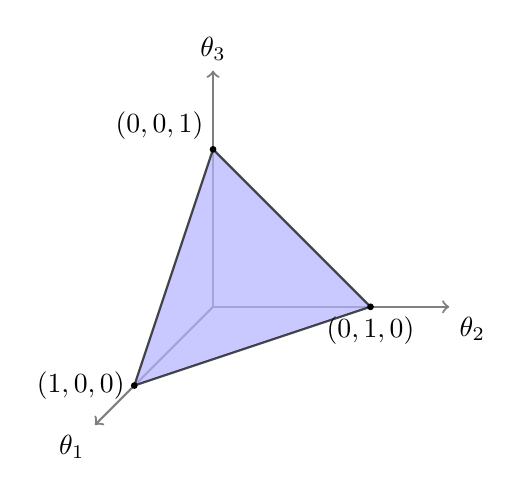
\begin{tikzpicture}[
    x={(-0.5cm,-0.5cm)}, 
    y={(1cm,0cm)}, 
    z={(0cm,1cm)}, 
    scale=2
]

    % Draw the axes
    \draw[->, thick, gray] (0,0,0) -- (1.5,0,0) node[anchor=north east, text=black] {$\theta_1$};
    \draw[->, thick, gray] (0,0,0) -- (0,1.5,0) node[anchor=north west, text=black] {$\theta_2$};
    \draw[->, thick, gray] (0,0,0) -- (0,0,1.5) node[anchor=south, text=black] {$\theta_3$};

    % Define the vertices of the simplex
    \coordinate (X) at (1,0,0);
    \coordinate (Y) at (0,1,0);
    \coordinate (Z) at (0,0,1);

    % Draw dashed lines from the origin to the vertices
    \draw[dashed, gray] (0,0,0) -- (X);
    \draw[dashed, gray] (0,0,0) -- (Y);
    \draw[dashed, gray] (0,0,0) -- (Z);

    % Draw the simplex plane (triangle)
    \draw[fill=blue!30, opacity=0.7, thick, join=round] (X) -- (Y) -- (Z) -- cycle;

    % Label the vertices
    \filldraw (X) circle (0.5pt) node[left] {$(1,0,0)$};
    \filldraw (Y) circle (0.5pt) node[below] {$(0,1,0)$};
    \filldraw (Z) circle (0.5pt) node[above left] {$(0,0,1)$};

\end{tikzpicture}
    \caption{The unit simplex for $R=3$.}
    \label{fig:unit_simplex}
\end{figure}

In practice one often wants to abide to these constraints. 
Therefore, \citet{FoxKimRyanBajari2011} suggest the following constrained least squares estimator
\begin{equation}
\label{eq:FKRBCLSest}
    \hat{\bm{\theta}}^{\mathrm{FKRB}} = \argmin_{\bm{\theta} \in \Delta_R}{\frac{1}{2NJ}\sum_{i=1}^{N}\sum_{j=1}^{J}(y_{ij}-\bm{z}^\prime_{ij}\bm{\theta})^2}.
\end{equation}
Under some additional regularity conditions, this estimator is also consistent \citep{Liew1976}.
One then tries to reconstruct $F_{0}$ according to
\begin{equation}
\label{eq:FKRBest}
    \hat{F}_{0}^{\mathrm{FKRB}}(\bm{b}) = \sum_{r=1}^R \left[\hat{\theta}^{\mathrm{FKRB}}_r \prod_{k=1}^{K}\mathds{1}{\{\beta^{r}_k < b_k\}}\right].
\end{equation}
We call this the FKRB estimator.\footnote{In the literature, the estimators in \cref{eq:FKRBCLSest,eq:FKRBest} are interchangeably called the FKRB estimator.}
The original FKRB estimator can be seen as a parametric estimator, since the estimator is determined merely by an $R$-dimensonial parameter vector, with prespecified $R < \infty$.
\subsubsection{Nonnegative LASSO estimator}
\label{sec:FKRBNNL}
\citet{HeissHetzeneckerOsterhaus2022} show the FKRB estimator can also be expressed as a nonnegative LASSO (NNL) estimator \citep[see][]{WuYangLiu2014,EfronHastieJohnstoneTibshirani2004}.
The NNL version is equivalent to the FKRB estimator, but does not need any quadratic programming to be computed, in contrast to the FKRB estimator.
The NNL estimator can be computed with coordinate descent, which is considerably faster than common quadratic programming solving procedures \citep{FriedmanHastieTibshirani2010}.
This makes it attractive to implement the FKRB estimator in the NNL form.

For completeness, we will also show the derivation of the equality of the NNL and FKRB estimator.
Consider constraints \eqref{eq:FKRBconstraint1} and \eqref{eq:FKRBconstraint2}.
Since the weights $\theta_r$ need to sum to one and each individual weight is nonnegative, we know, without loss of generality, that 
\begin{equation}
\label{eq:FKRBNNLthetaR}
    \theta_R = 1 - \sum_{r=1}^{R-1}\theta_r \geq 0.
\end{equation}
This means that under this identification we can rewrite constraints \eqref{eq:FKRBconstraint1} and \eqref{eq:FKRBconstraint2} into
\begin{align}
\label{eq:FKRBNNLconstraint1}
    &\sum_{r=1}^{R-1}\theta_r \leq 1, \\
\label{eq:FKRBNNLconstraint2}
    &\theta_r \geq 0, \text{ for all } r = 1,\ldots,R-1.
\end{align}

Now consider the objective function of \cref{eq:FKRBCLSest}.
Under the identification of \cref{eq:FKRBNNLthetaR} we can rewrite $y_{ij} - \bm{z}^\prime_{ij}\bm{\theta}$ as
\begin{align}
    y_{ij} - \bm{z}^\prime_{ij}\bm{\theta} & = y_{ij} - \sum_{r=1}^{R}\theta_r z_{ijr} = y_{ij} - \left(\sum_{r=1}^{R-1}\theta_r z_{ijr} +\theta_R z_{ijR}\right) \\
        &= y_{ij} - \left(\sum_{r=1}^{R-1}\theta_r z_{ijr} +\left(1 - \sum_{r=1}^{R - 1}\theta_r\right) z_{ijR}\right) \\
        &= y_{ij} - \left(\sum_{r=1}^{R-1}\theta_r z_{ijr} +z_{ijR} - \sum_{r=1}^{R - 1}\theta_r z_{ijR}\right) \\
        &= y_{ij} - \left(z_{ijR} + \sum_{r=1}^{R - 1}\theta_r (z_{ijr} -z_{ijR})\right) \\
        &= (y_{ij} - z_{ijR}) - \sum_{r=1}^{R - 1}\theta_r (z_{ijr} -z_{ijR}) \\
        &= \tilde{y}_{ij} - \tilde{\bm{z}}^\prime_{ij}\bm{\theta},
\end{align}
where $\tilde{y}_{ij} = y_{ij} - z_{ijR}$ and $\tilde{\bm{z}}_{ij} = (\tilde{z}_{ij1},\tilde{z}_{ij2},\ldots,\tilde{z}_{ij(R-1)})$ with $\tilde{z}_{ijr} = z_{ijr} -z_{ijR}$.

We can now reformulate \cref{eq:FKRBCLSest} into
\begin{equation}
\label{eq:FKRBNNLSestpart}
    \begin{split}
        \hat{\bm{\theta}}^{\mathrm{NNL*}} = &\argmin_{\bm{\theta}}{\frac{1}{2NJ}\sum_{i=1}^{N}\sum_{j=1}^{J}(\tilde{y}_{ij}-\tilde{\bm{z}}^\prime_{ij}\bm{\theta})^2}, \\
            &\text{ subject to constraints \eqref{eq:FKRBNNLconstraint1} and \eqref{eq:FKRBNNLconstraint2}}.
    \end{split}
\end{equation}
This is a NNL estimator with a pre-specified tuning parameter.
Unfortunately, \cref{eq:FKRBNNLSestpart} is formulated in the constrained optimization form, whereas most of the literature is specified in the Lagrangian form \citep[e.g.][]{WuYangLiu2014}.
Most solving algorithms are running on the Lagrangian formulation as well, such as the algorithms in scikit-learn \citep{scikitlearn2011} or glmnet \citep{FriedmanHastieTibshirani2010}.
Although, the tuning parameter in the constrained optimization form does have a one-to-one correspondence to the tuning parameter in the Lagrangian form, this correspondence is dependent on the data and not straightforward to calculate.

Note that $\hat{\bm{\theta}}^{\mathrm{NNL*}}$ only estimates the first $R-1$ terms. Therefore the complete estimator reads as
\begin{equation}
\label{FKRBNLSest}
    \hat{\bm{\theta}}^{\mathrm{NNL}} = \left(\hat{\bm{\theta}}^{\mathrm{NNL*}}, 1 - \sum_{r=1}^{R-1}\hat{\theta}^{\mathrm{NNL*}}_r\right).
\end{equation}
Since all we did was just rewriting the FKRB estimator, we have that $\hat{\bm{\theta}}^{\mathrm{FKRB}} = \hat{\bm{\theta}}^{\mathrm{NNL}}$.
\subsubsection{Feasible Generalized Least Squares}
\label{sec:FKRBGLS}
Up to this point the FKRB criterion has weighted each regression observation equally.
\citet{FoxKimRyanBajari2011} point out that this is statistically inefficient, because the error term $\zeta_{ij}$ defined in \cref{eq:FKRBzetadef} is both heteroskedastic in $\bm{x}_i$ and correlated across alternatives $j$ for the same individual $i$.

To see this, recall that $\zeta_{ij} = y_{ij} - \mathbb{P}(y_{ij} = 1 \mid \bm{x}_i)$.
Since $y_{ij}\in\{0,1\}$ and the vector $(y_{i1},\ldots,y_{iJ})^\prime$ contains at most one entry equal to one (the outside good absorbs the remaining mass), the moments of the stacked error $\bm{\zeta}_i = (\zeta_{i1},\ldots,\zeta_{iJ})^\prime$ are
\begin{align}
\label{eq:FKRBzetavar}
    \mathrm{Var}(\zeta_{ij}\mid \bm{x}_i) &= \mathbb{P}(y_{ij} = 1\mid \bm{x}_i)\bigl(1 - \mathbb{P}(y_{ij} = 1\mid \bm{x}_i)\bigr), \\
\label{eq:FKRBzetacov}
    \mathrm{Cov}(\zeta_{ij},\zeta_{ik}\mid \bm{x}_i) &= -\,\mathbb{P}(y_{ij} = 1\mid \bm{x}_i)\,\mathbb{P}(y_{ik} = 1\mid \bm{x}_i),\qquad j\neq k.
\end{align}
Collect these into the $J\times J$ matrix $\bm{\Omega}_i \coloneq \mathrm{Var}(\bm{\zeta}_i\mid \bm{x}_i)$.
Independence of $\bm{\zeta}_i$ across individuals then gives the $NJ\times NJ$ block-diagonal covariance matrix
\begin{equation}
\label{eq:FKRBOmega}
    \bm{\Omega} = \mathrm{diag}(\bm{\Omega}_1, \bm{\Omega}_2, \ldots, \bm{\Omega}_N).
\end{equation}
The infeasible optimally-weighted estimator is the generalized least squares (GLS) estimator
\begin{equation}
\label{eq:FKRBGLSest}
    \hat{\bm{\theta}}^{\mathrm{GLS}} = \argmin_{\bm{\theta} \in \Delta_R}\,(\bm{y} - \bm{Z}\bm{\theta})^\prime \bm{\Omega}^{-1}(\bm{y} - \bm{Z}\bm{\theta}).
\end{equation}
This is infeasible because $\bm{\Omega}$ depends on the unknown choice probabilities $\mathbb{P}(y_{ij} = 1 \mid \bm{x}_i)$, which themselves depend on $\bm{\theta}$.

\citet{FoxKimRyanBajari2011} therefore propose a two-step feasible procedure.
In the first step, compute the original identity-weighted FKRB estimator $\hat{\bm{\theta}}^{\mathrm{FKRB}}$ from \cref{eq:FKRBCLSest}.
In the second step, use it to form plug-in estimates of the choice probabilities
\begin{equation}
\label{eq:FKRBPhat}
    \hat{\mathbb{P}}(y_{ij} = 1 \mid \bm{x}_i) = \bm{z}_{ij}^\prime \hat{\bm{\theta}}^{\mathrm{FKRB}},
\end{equation}
substitute these into equations \eqref{eq:FKRBzetavar} and \eqref{eq:FKRBzetacov} to obtain $\hat{\bm{\Omega}}$, and solve
\begin{equation}
\label{eq:FKRBFGLSest}
    \hat{\bm{\theta}}^{\mathrm{FGLS}} = \argmin_{\bm{\theta} \in \Delta_R}\,(\bm{y} - \bm{Z}\bm{\theta})^\prime \hat{\bm{\Omega}}^{-1}(\bm{y} - \bm{Z}\bm{\theta}).
\end{equation}
Under standard regularity conditions $\hat{\bm{\theta}}^{\mathrm{FGLS}}$ is consistent and shares the asymptotic distribution of the infeasible $\hat{\bm{\theta}}^{\mathrm{GLS}}$ in \cref{eq:FKRBGLSest}, so the two-step procedure recovers the efficiency gain at no asymptotic cost \citep{Greene2019}.
\subsubsection{Nonparametric FKRB estimator}
\label{sec:nonparametricFKRB}
For the FKRB estimator proposed by \citet{FoxKimRyanBajari2011} the researcher prespecifies a fixed grid of $R$ support points.
Because of the a priori choice of a fixed grid, the estimator from \citet{FoxKimRyanBajari2011} has sometimes been called the fixed grid FKRB estimator in the subsequent literature \citep[see][]{FoxKimYang2016,HeissHetzeneckerOsterhaus2022}.
Since the performance of the estimator depends on the assumption $\tilde{\mathcal{B}} = \mathcal{B}$, the choice of the $R$ grid points should ideally equal the true support.
However, it is not reasonable to assume the researcher knows the true support $\mathcal{B}$.
When the researcher misspecifies the support, the fixed grid FKRB estimator becomes biased \citep{FoxKimYang2016}.

Intuitively, the researcher might tackle this problem by letting the grid become finer, which decreases the bias.
However, with a too fine grid the variance of the estimator will explode.
This is, at least partly, caused by the ``random'' weight selecting behavior of the estimator, which is observed in many empirical studies using the FKRB estimator \citep[such as][]{NevoTurnerWilliams2016,IllanesPadi2019,BlundellGowrisankaranLanger2020}.
This can be explained by the nonnegative LASSO specification of the estimator.
The LASSO estimator tends to ``randomly'' assign a positive probability mass to only one grid point in a cluster of highly correlated grid points \citep{HeissHetzeneckerOsterhaus2022}.
Since the grid points are closer to each other in a finer grid, the correlation between the points are also higher.
This increases the severity of the ``random'' selection problem, which in turn increases the variance.
This creates a classic bias-variance tradeoff.
However, since variance decreases at a higher rate than bias when $N \to \infty$, the optimal $R$ in a bias-variance sense increases with $N$.

\citet{FoxKimYang2016} acknowledge this and formulate a nonparametric variation on the FKRB estimator that allows $R$ to increase with $N$.
This variation is often called the nonparametric FKRB estimator.
For a fixed sample size $N$, their extension behaves the same as the fixed grid FKRB estimator.
This also has the implication that the finite-sample properties are the same.
However, when the sample size increases, they allow $R$ to increase as well.
This means that for their extension, the $R$ grid points are chosen \textit{a posteriori}, rather than being fixed \textit{a priori}.

The difference between these two versions is merely the theoretical paradigm on which these estimators rest.
After the choice of the $R$ grid points the estimators behave exactly the same.
The nonparametric estimator allows for new theoretical asymptotic results.
This estimator is namely a sieve estimator \citep[see][]{Chen2007}.
Here the grid of points, becoming increasingly dense in the true support as $N \to \infty$, induces the sieve basis.
The sieve approach for asymptotic theory is explored by \citet{FoxKimYang2016}.
To accentuate the dependence on $N$, we denote the nonparametric FKRB estimator as $\hat{\bm{\theta}}^{\mathrm{FKRB}}(N)$.

\subsubsection{Nonparametric FKRB as PSMD}
\label{sec:FKRBasPSMD}
We can be precise about the sieve structure by casting the nonparametric FKRB estimator in the PSMD form of \citet{ChenPouzo2012,ChenPouzo2015}.
We should note that, although we can write the FKRB estimator as a PSMD estimator in the sense of \citet{ChenPouzo2015}, we cannot directly use their inferential theory, as the FKRB estimator does not satisfy some of their regularity conditions.
We will highlight any mismatches between the FKRB estimator and these regularity conditions.

Let us start by writing FKRB in the SMD form \citep[see][]{AiChen2003}, the unpenalized special case of the PSMD estimator.
\citet{ChenPouzo2015} consider models specified by a conditional moment restriction of the form
\begin{equation}
\label{eq:CPcondmom}
    \mathbb{E}[\bm{\rho}(\bm{y}_i, \bm{x}_i; \alpha_0) \mid \bm{x}_i] = \bm{0}
\end{equation}
where $\bm{\rho} = (\rho_1,\rho_2,\ldots,\rho_J)$ is a $J$-dimensional function resembling generalized residuals and $\alpha_0$ is the (possibly infinite-dimensional) unknown parameter.
For the mixed logit we take $\alpha_0 = F_0$ and define
\begin{equation}
\label{eq:rhoMXL}
    \rho_j(\bm{y}_i, \bm{x}_i; F) = y_{ij} - \int_{\mathcal{B}} g_j(\bm{x}_i, \bm{\beta}) \, \mathrm{d}F(\bm{\beta}),
\end{equation}
for all $j$. By \cref{eq:mxlcondprob} we have that $\mathbb{E}[\rho_j(\bm{y}_i,\bm{x}_i; F_0) \mid \bm{x}_i] = 0$ for all $j$, so \cref{eq:CPcondmom} holds at $\alpha_0 = F_0$.
There is no finite-dimensional component to $\alpha_0$, so we are in the purely nonparametric case of \citet{ChenPouzo2015}.

The SMD estimator is then defined as the minimizer, over a sieve $\mathcal{A}_{R(N)}$, of an empirical criterion
\begin{equation}
\label{eq:SMDcrit}
    Q_N(\alpha) = \frac{1}{N}\sum_{i=1}^N \hat{\bm{m}}(\bm{x}_i, \alpha)^\prime\, \hat{\bm{\Sigma}}(\bm{x}_i)^{-1}\, \hat{\bm{m}}(\bm{x}_i, \alpha),
\end{equation}
where $\hat{\bm{m}}(\bm{x}, \alpha)$ is a nonparametric estimator of the conditional mean $\bm{m}(\bm{x}, \alpha) = \mathbb{E}[\bm{\rho}(\bm{y}, \bm{x}; \alpha) \mid \bm{x}]$, and $\hat{\bm{\Sigma}}(\bm{x})$ is a positive-definite weighting matrix.
To identify FKRB with this construction we need to specify the sieve, the conditional mean estimator $\hat{\bm{m}}$, and the weighting matrix $\hat{\bm{\Sigma}}$.

Let us start with the sieve.
The nonparametric FKRB estimator uses the linear sieve
\begin{equation}
\label{eq:FKRBsieve}
    \mathcal{A}_{R(N)} = \mathcal{F}_{R} = \left\{F_{\bm{\theta}} \;\middle|\; F_{\bm{\theta}}(\bm{b}) = \sum_{r=1}^{R} \left[\theta_r\prod_{k=1}^{K}\mathds{1}{\{\beta^{r}_k < b_k\}}\right]\!, \quad \bm{\theta} \in \Delta_{R}\right\},
\end{equation}
with both $R = R(N)$ and the grid points $\tilde{\mathcal{B}} = \{\bm{\beta}^{(1)}, \ldots, \bm{\beta}^{(R)}\}$ chosen by the researcher as a function of $N$. 
The sequence $\{\mathcal{F}_R\}_{R\in\mathbb{N}}$ grows dense in $\mathcal{F}$, the space of all distribution functions, as $N\to\infty$ and constitutes a sieve in the sense of \citet{Chen2007}.
We flag one structural caveat already here.
The basis functions $\prod_{k=1}^{K}\mathds{1}\{\beta^{r}_k < b_k\}$ are linear in the coefficients, but the admissible coefficients are confined to the unit simplex $\Delta_R$, so $\mathcal{F}_R$ is a convex polytope, not the closed linear subspace required by \citet[][Assumption~3.1(ii)]{ChenPouzo2015}.
The inequality constraints $\theta_r\ge 0$ that separate $\Delta_R$ from its linear span are precisely what place FKRB outside their framework, and what generate the boundary phenomena discussed in \Cref{sec:Inference}.
On the sieve $\rho_j$ is linear in $\bm{\theta}$:
\begin{equation}
\label{eq:rhoMXLsieve}
    \rho_j(\bm{y}_i, \bm{x}_i; F_{\bm{\theta}}) = y_{ij} - \sum_{r=1}^R \theta_r\, g_j(\bm{x}_i, \bm{\beta}^{(r)}) = y_{ij} - \bm{z}_{ij}^\prime \bm{\theta},
\end{equation}
recovering exactly the regression design in \cref{eq:FKRBzetadef}.

Let us now look at the conditional mean estimator $\hat{\bm{m}}$ and the weighting matrix $\hat{\bm{\Sigma}}$.
Take the trivial $\hat{\bm{m}}(\bm{x}_i, F) = \bm{\rho}(\bm{y}_i, \bm{x}_i; F)$, that is, do no smoothing of $\bm{\rho}$, and take the identity weighting $\hat{\bm{\Sigma}}(\bm{x}_i) = \bm{I}_J$.
The criterion \cref{eq:SMDcrit} then reduces to
\begin{equation}
\label{eq:FKRBPSMDcrit}
    Q_N(F) = \frac{1}{N}\sum_{i=1}^N\sum_{j=1}^J \rho_j(\bm{y}_i,\bm{x}_i; F)^2,
\end{equation}
and restricting $F$ to $\mathcal{F}_R$ via \cref{eq:rhoMXLsieve} gives
\begin{equation}
\label{eq:FKRBPSMDcritsieve}
    Q_N(F_{\bm{\theta}}) = \frac{1}{N}\sum_{i=1}^N\sum_{j=1}^J (y_{ij} - \bm{z}_{ij}^\prime\bm{\theta})^2,
\end{equation}
which is $2J$ times the FKRB objective in \cref{eq:FKRBCLSest}.
Minimizing $Q_N$ over $\mathcal{F}_R$ therefore yields the constrained FKRB estimator $\hat{\bm{\theta}}^{\mathrm{FKRB}}$.
We write
\begin{equation}
\label{eq:SMDdef}
    \hat{\bm{\theta}}^{\mathrm{SMD}}(N) \coloneq \argmin_{F_{\bm{\theta}} \in \mathcal{F}_R} {Q_N(F_{\bm{\theta}})} = \hat{\bm{\theta}}^{\mathrm{FKRB}}(N).
\end{equation}

We should add that $\bm{I}_J$ is not the optimal weighting matrix in the SMD framework.
\citet{ChenPouzo2015} call the SMD estimator optimally weighted when $\hat{\bm{\Sigma}}(\bm{x}_i)$ is a consistent estimator of
\begin{equation}
\label{eq:Sigma0def}
    \bm{\Sigma}_0(\bm{x}_i) \coloneq \mathrm{Var}\bigl(\bm{\rho}(\bm{y}_i, \bm{x}_i; \alpha_0)\mid \bm{x}_i\bigr).
\end{equation}
At $\alpha_0 = F_0$ the residual reduces to $\rho_j(\bm{y}_i, \bm{x}_i; F_0) = \zeta_{ij}$ from \cref{eq:FKRBzetadef}, so
\begin{equation}
\label{eq:FKRBSigma0equalsOmega}
    \bm{\Sigma}_0(\bm{x}_i) = \mathrm{Var}(\bm{\zeta}_i \mid \bm{x}_i) = \bm{\Omega}_i,
\end{equation}
which is exactly the $i$th $J\times J$ block of the GLS covariance matrix \cref{eq:FKRBOmega} from \Cref{sec:FKRBGLS}.
Plugging $\bm{\Omega}_i$ into the SMD criterion \cref{eq:SMDcrit} reproduces, up to a factor of $\frac{1}{N}$, the infeasible GLS objective \cref{eq:FKRBGLSest}, and substituting the first-stage plug-in estimate $\hat{\bm{\Omega}}_i$ reproduces the feasible GLS objective \cref{eq:FKRBFGLSest}.
The feasible GLS estimator $\hat{\bm{\theta}}^{\mathrm{FGLS}}$ of \Cref{sec:FKRBGLS} therefore matches the optimally-weighted SMD estimator for this model.

We conclude that the constrained nonparametric FKRB estimator can be written in the SMD form of \citet{ChenPouzo2015}, with sieve $\mathcal{F}_R$, trivial conditional-mean estimator, and identity weighting.
However, because of the caveat that the FKRB sieve $\mathcal{A}_{R(N)}$ does not satisfy the regularity conditions of \citet{ChenPouzo2015}, we cannot directly import their results.
The value of the form is that the criterion $Q_N$ coincides with their (P)SMD expressions.
Therefore we can show that their sieve Wald and QLR statistics coincide with ours.
More generally, one can also write this as a PSMD estimator:
\begin{equation}
\label{eq:PSMDdef}
    \hat{\bm{\theta}}^{\mathrm{PSMD}}(N) \coloneq \argmin_{F_{\bm{\theta}} \in \mathcal{F}_R} {Q_N(F_{\bm{\theta}}) + \lambda_N \mathrm{Pen}(F_{\bm{\theta}})} = \hat{\bm{\theta}}^{\mathrm{SMD}}(N) = \hat{\bm{\theta}}^{\mathrm{FKRB}}(N),
\end{equation}
with $\lambda_N = 0$ and $\mathrm{Pen}(\cdot)$ an arbitrary penalty function.
The elastic net extension of \citet{HeissHetzeneckerOsterhaus2022} fits better in this framework, as the regularization performed by the elastic net can correspond to the penalty part of the PSMD estimator.

FKRB can equivalently be cast as a sieve M-estimator with squared-loss objective.
Define the population objective $L(F) = \mathbb{E}[\sum_{j=1}^J(y_{ij} - \int_{\mathcal{B}} g_j(\bm{x}_i,\bm{\beta})\,\mathrm{d}F(\bm{\beta}))^2]$ and minimize its sample analog over $\mathcal{F}_R$.
The two criteria coincide here because of the choice of trivial $\hat{\bm{m}}$ and identity weighting in \cref{eq:FKRBPSMDcrit}.
This equivalence would break under, for example, the optimally-weighted choice $\hat{\bm{\Sigma}}(\bm{x}_i) = \hat{\bm{\Omega}}_i$, where FKRB becomes a feasible-GLS variant of the SMD criterion that no longer corresponds to a pure least-squares M-estimator.
The M-estimator characterization might allow for an application of \citet{Li2025The,Li2025Inference}, but that is not in the scope of this thesis.
We will keep our focus on the PSMD characterization, since the sieve Wald and QLR statistics of \citet{ChenPouzo2015}, to which we will compare our test statistics, are written for PSMD estimators. 

A central object in their machinery is the sieve variance $||v^*_n||_{\mathrm{sd}}$ of a smooth functional $T:\mathcal{F}\to\mathbb{R}$, which captures the asymptotic spread of the plug-in PSMD estimator $\hat{\eta} \coloneq T(F_{\hat{\bm{\theta}}^{\mathrm{PSMD}}})$.
\citet[][eq.~(2.10)]{ChenPouzo2015} define a consistent estimator for it by the delta-method sandwich
\begin{equation}
\label{eq:sievevariance}
    \|\hat{v}^*_n\|^2_{\mathrm{sd}} \coloneq N\nabla T\!\bigl(\hat{\bm{\theta}}^{\mathrm{PSMD}}\bigr)^\prime\, \hat{\bm{H}}^{-1}\, \hat{\bm{V}}\, \hat{\bm{H}}^{-1}\, \nabla T\!\bigl(\hat{\bm{\theta}}^{\mathrm{PSMD}}\bigr),
\end{equation}
where
\begin{equation}
\label{eq:sieveinformation}
    \hat{\bm{H}} = \sum_{i=1}^{N}\hat{\bm{D}}_i^\prime\hat{\bm{\Sigma}}_i^{-1}\hat{\bm{D}}_i,\qquad \hat{\bm{D}}_i = \left.\frac{\partial \hat{\bm{m}}(\bm{x}_i,F_{\bm{\theta}})}{\partial \bm{\theta}^\prime}\right|_{\bm{\theta} = \hat{\bm{\theta}}^{\mathrm{PSMD}}},
\end{equation}
is the sieve Fisher information, with $\hat{\bm{D}}_i$ collecting the moment-residual sensitivities at the estimate, and
\begin{equation}
\label{eq:sievescorevariance}
    \hat{\bm{V}} = \sum_{i=1}^{N}\bm{s}_i\bm{s}_i^\prime,\qquad \bm{s}_i = \hat{\bm{D}}_i^\prime\hat{\bm{\Sigma}}_i^{-1}\hat{\bm{m}}\!\bigl(\bm{x}_i, F_{\hat{\bm{\theta}}^{\mathrm{PSMD}}}\bigr),
\end{equation}
is the outer product of the individual-$i$ moment scores evaluated at the estimate.
The leading and trailing factors $\nabla T(\hat{\bm{\theta}}^{\mathrm{PSMD}})$ propagate the resulting parameter variance to the scalar functional in the standard delta-method way.
Under the regularity conditions of \citet{ChenPouzo2015}, $\|\hat{v}^*_n\|^2_{\mathrm{sd}}/N$ is a consistent estimator of the asymptotic variance of $\hat{\eta}$.
This consistency is what underpins the sieve Wald and QLR result in \citet[theorems~4.2 and 4.3]{ChenPouzo2015}.

\subsection{Inference}
\label{sec:Inference}
After having done the estimation procedure, the researcher often wants to conduct inference on $\hat{\bm{\theta}}^{\mathrm{FKRB}}$.
However it turns out that this is not at all trivial for this estimator.
Because of the constrained nature of the estimator, it is hard to establish an asymptotic distribution, let alone a finite-sample distribution.
For many estimators, central limit theorems can do a lot of heavy lifting in establishing at least the asymptotic distribution, which is then often Gaussian.
However, when the true parameter is on the boundary, asymptotic normality breaks down \citep{Andrews1999}.
These results however are unfortunately not general enough to also apply to the FKRB estimator \citep{FoxKimRyanBajari2011}.

A seemingly related problem is the Hauck-Donner effect \citep{HauckDonner1977}, which is observed in the binary logit model.
This effect describes that the variance of the estimator for the probability parameter blows up near the boundary.
However, this does not apply here, because the FKRB standard errors come from the sandwich variance of a least-squares regression, not from the inverse Fisher information of a binomial likelihood.
The boundary-induced variance blowup that drives the Hauck-Donner effect is specific to the binomial Fisher information; the sandwich variance is controlled by the regression residuals $\hat{\zeta}_{ij}$ and does not exhibit this pathology.

This subsection will focus on inference procedures for the FKRB estimator.

\subsubsection{Confidence intervals}
\label{sec:confidenceintervals}
Inference on the FKRB estimator is done with confidence intervals.
We will first need a rigorous framework to analyze empirical confidence intervals in the upcoming sections.
This subsection presents such a framework.

Let $\bm{X} = (X_1, X_2, \ldots, X_n)$ be a random sample from a distribution that depends on a parameter $\theta$.
Let $L(\bm{X}), U(\bm{X})$ be two statistics such that $L(\bm{X}) \leq U(\bm{X})$. Then $\mathrm{CI}_{1-\alpha,\theta}(\bm{X}) = [L(\bm{X}),U(\bm{X})]$ is defined to be a confidence interval for $\theta$ at the $\alpha$ significance level and $1-\alpha$ confidence level if and only if\footnote{For brevity we will hereafter simply denote $\mathrm{CI}_{1-\alpha,\theta}(\bm{X}) = \mathrm{CI}_{1-\alpha,\theta}$.}
\begin{equation}
\label{eq:confidenceinterval}
    \mathbb{P}(\theta \in \mathrm{CI}_{1-\alpha,\theta}) \geq 1- \alpha
\end{equation}

Some authors impose an equality sign in \cref{eq:confidenceinterval}.
However, this would exclude the possibility of a conservative confidence interval.
We call a confidence interval conservative if the inequality in \cref{eq:confidenceinterval} is non-binding, that is
\begin{equation}
\label{eq:conservativeconfidenceinterval}
    \mathbb{P}(\theta \in \mathrm{CI}_{1-\alpha,\theta}) > 1- \alpha.
\end{equation}
The binomial proportion Clopper-Pearson confidence interval \citep{ClopperPearson1934} is an example of a highly conservative confidence interval in the literature \citep[see also][]{BrownCaiDasGupta2001}.
Conservative intervals are also observed by \citet{Garwood1936,Dunn1959,Dunn1961}.
We will soon see that the confidence intervals in \Cref{sec:FKRBconfidence} are also examples of conservative confidence intervals \citep{FoxKimRyanBajari2011}.

Conservative confidence intervals are generally undesirable because they reduce statistical power. 
In standard hypothesis testing, a researcher sets a nominal significance level and rejects the null hypothesis if the corresponding interval excludes the null value. 
However, because conservative intervals are wider than exact intervals, they increase the risk of a Type II error.
This means the researcher might fail to reject a null hypothesis that an exact interval would have successfully rejected.

Therefore, we want to measure the ``conservativeness'' of confidence intervals.
One way to do this is by comparing the nominal coverage probability $1 - \alpha$ with the true or empirical coverage $c_{\mathrm{CI}_{1-\alpha,\theta}}(\theta) = \mathbb{P}(\theta \in \mathrm{CI}_{1-\alpha,\theta})$ of $\mathrm{CI}_{1-\alpha,\theta}$ when $\theta$ is the true parameter.
Note that $c_{\mathrm{CI}_{1-\alpha,\theta}}(\theta)$ can vary for different $\theta$ in the parameter space.

\subsubsection{FKRB confidence intervals}
\label{sec:FKRBconfidence}

\citet{FoxKimRyanBajari2011} have suggested an inference procedure themselves.
Their method is based on the Wald's test \citep{Wald1943}.
They construct an initial confidence interval $\mathrm{CI}^{*}_{1-\alpha, \theta_r}$ at the $\alpha$ significance level for $\theta_r$ with heteroskedasticity-robust standard errors that arise from the unconstrained OLS estimator $\hat{\bm{\theta}}^{\mathrm{OLS}}$ from \cref{eq:FKRBOLSest}.
The need of heteroskedasticity-robust standard errors comes from the inherent heteroskedasticity introduced by the construction of the error term $\zeta_{ij}$ in \cref{eq:FKRBzetadef}.
There are also clear clusters (each individual has one), so they also cluster the standard errors at the level of ``regression observations'' $j = 1,\ldots,J$ for each individual $i$.
\citet{FoxKimRyanBajari2011} do not specify a specific way of calculating the robust standard errors.
We will estimate the variance-covariance matrix of $\hat{\bm{\theta}}^{\mathrm{OLS}}$ with the cluster-robust sandwich estimator of \citet{LiangZeger1986},
\begin{equation}
\label{eq:FKRBclustervcov}
    \widehat{\mathrm{Var}}\!\left(\hat{\bm{\theta}}^{\mathrm{OLS}}\right) = c_{N,J,R}\,(\bm{Z}^\prime\bm{Z})^{-1}\!\left(\sum_{i=1}^{N} \bm{s}_i \bm{s}_i^\prime\right)\!(\bm{Z}^\prime\bm{Z})^{-1},
\end{equation}
with $\bm{s}_i = \sum_{j=1}^{J} \bm{z}_{ij}\,\hat{\zeta}_{ij}^{\mathrm{OLS}}$ the individual-$i$ cluster score evaluated at the unconstrained residuals $\hat{\zeta}_{ij}^{\mathrm{OLS}} = y_{ij} - \bm{z}_{ij}^\prime \hat{\bm{\theta}}^{\mathrm{OLS}}$.
The scalar $c_{N,J,R}$ is the standard finite-sample bias correction recommended by \citet{CameronMiller2015} (commonly referred to as the CR1 correction):
\begin{equation}
\label{eq:FKRBclusterbc}
    c_{N,J,R} = \frac{N}{N-1}\cdot\frac{NJ-1}{NJ-R}.
\end{equation}
This inflation factor converges to one as $N\to\infty$, but corrects for the downward bias of the naive plug-in sandwich at small $N$.
The standard error $\mathrm{SE}(\hat{\theta}_r^{\mathrm{OLS}})$ used in \cref{eq:CIOLS} below is then the square root of the $r$-th diagonal element of \cref{eq:FKRBclustervcov}.

Formally, we have
\begin{equation}
\label{eq:CIOLS}
    \mathrm{CI}^{*}_{1-\alpha,\theta_r} = \left[\hat{\theta}_{r}^{\mathrm{OLS}} - z_{1-\frac{\alpha}{2}}\mathrm{SE}\left(\hat{\theta}_{r}^{\mathrm{OLS}}\right),\hat{\theta}_{r}^{\mathrm{OLS}} + z_{1-\frac{\alpha}{2}}\mathrm{SE}\left(\hat{\theta}_{r}^{\mathrm{OLS}}\right)\right],
\end{equation}
where $z_{1-\frac{\alpha}{2}} = \Phi^{-1}(1-\frac{\alpha}{2})$ denotes the $1-\frac{\alpha}{2}$ quantile of the standard normal distribution and $\mathrm{SE}(\hat{\theta}_{r}^{\mathrm{OLS}})$ denotes the clustered heteroskedasticity-robust standard error of $\hat{\theta}_{r}^{\mathrm{OLS}}$.
Note that both the centre point and the width of the interval is determined by the OLS estimator and its clustered heteroskedasticity-robust standard errors.
However, the interval has correct coverage for both the unconstrained OLS estimator and the constrained FKRB estimator \citep{AndrewsGuggenberger2010Applications,FoxKimRyanBajari2011}.

It is also good to note that this method acts as if the estimator is asymptotically normally distributed. 
Although this is wrong at the boundary \citep{Andrews1999}, asymptotic normality in the interior has been proven for broad classes of PSMD estimators \citep{ChenPouzo2015}, but unfortunately these classes exclude the FKRB estimator.
However, \citet[page~241]{FoxKimYang2016} conjecture that asymptotic normality does hold in the interior. 
Of course \cref{eq:CIOLS} allows for confidence intervals that cross outside the $[0,1]$ region, while this is clearly not possible for the real parameters as illustrated by \cref{eq:FKRBconstraint1,eq:FKRBconstraint2}.
The final interval that \citet{FoxKimRyanBajari2011} arrive at is therefore clipped to this region, i.e. 
\begin{equation}
\label{eq:CIFKRB}
    \mathrm{CI}^{\mathrm{FKRB}}_{1-\alpha,\theta_r} = [0,1] \cap \mathrm{CI}^{*}_{1-\alpha, \theta_r}.
\end{equation}
The clipping cannot decrease the empirical coverage.
Therefore the clipped interval retains correct coverage.
However, it may reduce the width of the interval.

Even though the coverage may be correct, it can still be highly conservative.
In fact, it is.
\citet{FoxKimRyanBajari2011} noticed that the confidence intervals had a much higher empirical coverage than their nominal coverage.
Tikhonov regularization reduced this somewhat.
\citet{HeissHetzeneckerOsterhaus2022} show that much less grid points are estimated to have a probability mass of zero when regularization is applied.
This results in less grid points that are estimated to be on the boundary.
This hints in the direction that the conservativeness is higher on or close to the boundary.

When the researcher is interested in inference on a parameter $\eta$ determined by a single-valued functional $T$ on $\bm{\theta}$, i.e. $\eta = T(\bm{\theta})$, \citet{FoxKimRyanBajari2011} propose an adjusted procedure.
They scale the clipping interval to be the interval between the minimum and the maximum of $T(\bm{\theta})$ on the constraint set $\Delta_R$.
Since $\Delta_R$ is compact, by the Weierstrass extreme value theorem, the minimum and maximum are well-defined here if $T$ is continuous.
Furthermore they calculate $\mathrm{SE}(T(\hat{\bm{\theta}}^{\mathrm{OLS}}))$ with the multivariate delta method. That is
\begin{equation}
\label{eq:FKRBdeltamethod}
    \mathrm{SE}\left(T(\hat{\bm{\theta}}^{\mathrm{OLS}})\right) = \left[\nabla T\left(\hat{\bm{\theta}}^{\mathrm{OLS}}\right)^\prime \widehat{\mathrm{Var}}\left(\hat{\bm{\theta}}^{\mathrm{OLS}}\right) \nabla T\left(\hat{\bm{\theta}}^{\mathrm{OLS}}\right)\right]^{\frac{1}{2}}.
\end{equation}
The confidence interval $\widetilde{\mathrm{CI}}^{\mathrm{FKRB}}_{1-\alpha, \eta}$ for $\eta$ at the $\alpha$ significance level then becomes\footnote{We add a tilde to make clear that this is a different construction than $\mathrm{CI}_{\alpha,\theta_r}^{\mathrm{FKRB}}$.}
\begin{multline}
\label{eq:CIfunctional}
    \widetilde{\mathrm{CI}}^{\mathrm{FKRB}}_{1-\alpha,\eta} = \left[\min_{\bm{\theta}\in \Delta_R}{T(\bm{\theta})},\max_{\bm{\theta}\in \Delta_R}{T(\bm{\theta})}\right] \\
        \cap \left[\hat{\eta} -  z_{1-\frac{\alpha}{2}}\mathrm{SE}\left(T\left(\hat{\bm{\theta}}^{\mathrm{OLS}}\right)\right), \hat{\eta} +  z_{1-\frac{\alpha}{2}}\mathrm{SE}\left(T\left(\hat{\bm{\theta}}^{\mathrm{OLS}}\right)\right)\right],
\end{multline}
where $\hat{\eta} = T(\hat{\bm{\theta}}^\mathrm{OLS})$ denotes the plug-in estimator for $\eta$.

Notice that $\widetilde{\mathrm{CI}}^{\mathrm{FKRB}}_{1-\alpha,\eta} = \mathrm{CI}^{\mathrm{FKRB}}_{1-\alpha,\theta_r}$ when $\eta = T(\bm{\theta})$ is the select-$r$ functional.\footnote{This functional is denoted by $T: \mathbb{R}^R \to \mathbb{R}$ with $T(\bm{\theta}) = \bm{e}'_r \bm{\theta}$. Here $\bm{e}_r$ denotes the $r$th standard basis vector.}
Hence, you can see $\widetilde{\mathrm{CI}}^{\mathrm{FKRB}}_{1-\alpha,\eta}$ as the generalized version of $\mathrm{CI}^{\mathrm{FKRB}}_{1-\alpha,\theta_r}$.
\citet{ChenPouzo2015} is written in a similar generalized framework.
Therefore, we will use the generalized version to compare with \citet{ChenPouzo2015}.

\subsubsection{FKRB confidence intervals in the PSMD framework}
The interval $\widetilde{\mathrm{CI}}^{\mathrm{FKRB}}_{1-\alpha,\eta}$ is similar to the sieve Wald confidence interval for the functional $\eta = T(F_{\bm{\theta}})$ that can be constructed from the results of \citet[][theorem~4.2]{ChenPouzo2015}.
\citet{ChenPouzo2015} provide a way to estimate the variance of the FKRB estimator in the sense of the sieve variance $\|v^*_n\|_{\mathrm{sd}}$.
Therefore both the center and the width of the interval can be determined by the constrained FKRB estimator, in constrast to the FKRB confidence intervals which use the unconstrained OLS estimators for both the center and the width.
Their construction takes the form
\begin{equation}
\label{eq:CIChenPouzo}
    \mathrm{CI}^{\mathrm{CP}}_{1-\alpha, \eta} = \left[\hat{\eta} - z_{1-\frac{\alpha}{2}}\,\frac{\|\hat{v}^*_n\|_{\mathrm{sd}}}{\sqrt{N}},\ \hat{\eta} + z_{1-\frac{\alpha}{2}}\,\frac{\|\hat{v}^*_n\|_{\mathrm{sd}}}{\sqrt{N}}\right],
\end{equation}
where $\hat{\eta} = T(\hat{\bm{\theta}}^{\mathrm{PSMD}}) = T(\hat{\bm{\theta}}^{\mathrm{FKRB}})$ is the plug-in PSMD estimator and $\|\hat{v}^*_n\|^2_{\mathrm{sd}}$ is the estimated sieve variance of \citet[][eq.~2.10]{ChenPouzo2015}, see \cref{eq:sievevariance}.
We can decrease the width of the interval, while keeping coverage equal, by clipping the interval to $[\min_{\bm{\theta}\in \Delta_R}{T(\bm{\theta})},\max_{\bm{\theta}\in \Delta_R}{T(\bm{\theta})}]$.

Specializing \cref{eq:sievevariance} to the FKRB setting amounts to evaluating each of its three ingredients --- the moment-residual sensitivity $\hat{\bm{D}}_i$, the weighting $\hat{\bm{\Sigma}}_i^{-1}$, and the residual $\hat{\bm{m}}(\bm{x}_i, F_{\hat{\bm{\theta}}^{\mathrm{PSMD}}})$ --- and then substituting back.
Collect the rows $\bm{z}_{ij}^\prime$ of \cref{eq:FKRBzetadef} for $j=1,\ldots,J$ into a per-individual block $\bm{Z}_i \in \mathbb{R}^{J\times R}$.
Stacking these blocks vertically across $i=1,\ldots,N$ recovers the full $NJ\times R$ design matrix $\bm{Z}$ of \cref{eq:FKRBOLSest}.
Because $\hat{\bm{m}}$ is the trivial estimator in \cref{eq:FKRBPSMDcrit}, the moment $\hat{\bm{m}}(\bm{x}_i, F_{\bm{\theta}})$ coincides with the per-individual residual vector $\bm{\rho}_i(\bm{\theta}) = \bm{y}_i - \bm{Z}_i\bm{\theta}$, where $\bm{y}_i = (y_{i1},\ldots,y_{iJ})^\prime$.
Linearity of $\bm{\rho}_i$ in $\bm{\theta}$ then makes the sensitivity constant in $\bm{\theta}$:
\begin{equation}
\label{eq:Dihatfkrb}
    \hat{\bm{D}}_i = \left.\frac{\partial \hat{\bm{m}}(\bm{x}_i,F_{\bm{\theta}})}{\partial \bm{\theta}^\prime}\right|_{\bm{\theta} = \hat{\bm{\theta}}^{\mathrm{FKRB}}} = -\bm{Z}_i.
\end{equation}
Identity weighting $\hat{\bm{\Sigma}}_i = \bm{I}_J$ further simplifies the sieve Fisher information \cref{eq:sieveinformation} to
\begin{equation}
\label{eq:Hhatfkrb}
    \hat{\bm{H}} = \sum_{i=1}^N \bm{Z}_i^\prime \bm{Z}_i = \bm{Z}^\prime\bm{Z},
\end{equation}
since the block-wise sum reconstructs the Gram matrix of the stacked design $\bm{Z}$.
Evaluating $\hat{\bm{m}}$ at the PSMD estimate $\hat{\bm{\theta}}^{\mathrm{PSMD}} = \hat{\bm{\theta}}^{\mathrm{FKRB}}$ produces the per-individual constrained-residual vector $\hat{\bm{\zeta}}_i^{\mathrm{FKRB}} = \bm{y}_i - \bm{Z}_i\hat{\bm{\theta}}^{\mathrm{FKRB}}$ with components $\hat{\zeta}_{ij}^{\mathrm{FKRB}} = y_{ij} - \bm{z}_{ij}^\prime \hat{\bm{\theta}}^{\mathrm{FKRB}}$, so the individual-$i$ moment score in \cref{eq:sievescorevariance} reads
\begin{equation}
\label{eq:sifkrb}
    \bm{s}_i = \hat{\bm{D}}_i^\prime\, \hat{\bm{\Sigma}}_i^{-1}\,\hat{\bm{m}}\bigl(\bm{x}_i,F_{\hat{\bm{\theta}}^{\mathrm{FKRB}}}\bigr) = -\bm{Z}_i^\prime\,\hat{\bm{\zeta}}_i^{\mathrm{FKRB}} = -\sum_{j=1}^J \bm{z}_{ij}\,\hat{\zeta}_{ij}^{\mathrm{FKRB}}.
\end{equation}
The overall sign of $\bm{s}_i$ enters the sandwich only through the outer product $\bm{s}_i\bm{s}_i^\prime$ and is therefore immaterial; absorbing it, we redefine $\bm{s}_i \coloneq \sum_{j=1}^J \bm{z}_{ij}\,\hat{\zeta}_{ij}^{\mathrm{FKRB}}$ for the remainder.
Plugging $\hat{\bm{H}} = \bm{Z}^\prime\bm{Z}$ and $\hat{\bm{V}} = \sum_{i=1}^N \bm{s}_i\bm{s}_i^\prime$ into \cref{eq:sievevariance} and dividing by $N$ --- recall from the discussion below \cref{eq:sievevariance} that $\|\hat{v}_n^*\|^2_{\mathrm{sd}}/N$ is the relevant estimator of $\mathrm{Avar}(\hat{\eta})$ under \citet[][theorem~4.2]{ChenPouzo2015} --- yields the cluster-robust delta-method sandwich
\begin{equation}
\label{eq:CPsievevariance}
    \frac{\|\hat{v}^*_n\|^2_{\mathrm{sd}}}{N} = \nabla T\!\bigl(\hat{\bm{\theta}}^{\mathrm{FKRB}}\bigr)^\prime (\bm{Z}^\prime\bm{Z})^{-1}\!\left(\sum_{i=1}^N \bm{s}_i\bm{s}_i^\prime\right)\!(\bm{Z}^\prime\bm{Z})^{-1}\, \nabla T\!\bigl(\hat{\bm{\theta}}^{\mathrm{FKRB}}\bigr).
\end{equation}
By construction, $\hat{\bm{H}}^{-1}$ scales as $\mathcal{O}_p(1/N)$ and $\hat{\bm{V}}$ scales as $\mathcal{O}_p(N)$, meaning the sandwich $\hat{\bm{H}}^{-1}\hat{\bm{V}}\hat{\bm{H}}^{-1}$ scales as $\mathcal{O}_p(1/N)$. 
Multiplying this sandwich by $N$ isolates the $\mathcal{O}_p(1)$ sieve variance $\|\hat{v}_n^*\|^2_{\mathrm{sd}}$, consistent with the conventions adopted in \cref{eq:sievevariance,eq:sieveinformation,eq:sievescorevariance}.

The right-hand side of \cref{eq:CPsievevariance} is precisely the FKRB delta-method variance in \cref{eq:FKRBdeltamethod}, up to two implementation details.
First, \citet{ChenPouzo2015} evaluate the sieve variance at the constrained estimator $\hat{\bm{\theta}}^{\mathrm{PSMD}} = \hat{\bm{\theta}}^{\mathrm{FKRB}}$, whereas \citet{FoxKimRyanBajari2011} evaluate both the gradient $\nabla T$ and the sandwich residuals at the unconstrained $\hat{\bm{\theta}}^{\mathrm{OLS}}$.
When the true $\bm{\theta}_0$ lies in the interior of $\Delta_R$, the constraints are slack with probability approaching one, the constrained and unconstrained estimators are asymptotically equivalent, and the two variances agree to first order, so this choice has no first-order consequence.
On the boundary, however, the constrained and unconstrained estimators have different limiting distributions \citep{Andrews1999}.
The equivalence claimed here is therefore an interior statement only.
The second major difference between the two intervals is the center point.
Where FKRB use the unconstrained OLS estimator as center point, \citet{ChenPouzo2015} allows for the constrained FKRB estimator as center point.
Asymptotically, both the width and the center of the interval are equal, and therefore the intervals are asymptotically equal.

We repeat the comment that FKRB does not satisfy the regularity conditions of \citet{ChenPouzo2015}.
Therefore, even though we do rely on the results of \citet[theorem~4.2]{ChenPouzo2015}, we cannot be sure if they fully apply to the FKRB estimator.
In fact, we may expect that the asymptotic normality does not hold at the boundary.
\subsubsection{Sieve QLR confidence intervals}
\label{sec:QLRCI}
Both $\widetilde{\mathrm{CI}}^{\mathrm{FKRB}}_{1-\alpha,\eta}$ and its sieve Wald counterpart $\mathrm{CI}^{\mathrm{CP}}_{1-\alpha,\eta}$ require an explicit estimate of the asymptotic variance of $\hat{\eta}$ and must be intersected with the feasible range of $T$ in order to respect the simplex constraint.
An alternative construction that avoids both of these requirements is the sieve quasi-likelihood ratio (QLR) interval of \citet[][sec.~4.3]{ChenPouzo2015}, which inverts a test statistic that, under the suitable regularity conditions and optimal weighting, is asymptotically pivotal against a $\chi^2_1$ distribution and whose inversion is automatically confined to the feasible range of $T$.
Specifically the regularity conditions are again not met for the FKRB estimator, but the $\chi_1^2$-result possibly remains a good approximation.
For the fixed grid $R$ and a regular functional, $\mathrm{QLR}_N$ is nothing other than the classical criterion-difference (distance-metric) statistic of parametric minimum distance/GMM \citep[see][sec.~9]{NeweyMcFadden1994}, and the limit results \cref{eq:QLRoptimal,eq:QLRnonoptimal} below are the corresponding Wilks and studentized-Wilks theorems.
The sieve formulation of \citet{ChenPouzo2015} becomes essential only when the grid grows with $N$ or the functional is irregular.
The former only occurs in the nonparametric case.
The latter only occurs in special cases, not in the cases we will study.
A regular parametric QLR interval in the sense of \citet{NeweyMcFadden1994} is therefore not merely an adequate substitute here --- for the fixed grid it is exactly what \cref{eq:CIQLR} computes.

The construction compares the unrestricted minimum of the SMD criterion to its minimum subject to the null restriction $T(F_{\bm{\theta}}) = \eta_0$.
Let $Q_N$ denote the SMD criterion in \cref{eq:SMDcrit}, let
\begin{equation}
\label{eq:thetaRestricted}
    \hat{\bm{\theta}}^{R}(\eta_0) \coloneq \argmin_{\bm{\theta}\in\Delta_R\,:\,T(\bm{\theta}) = \eta_0} Q_N(F_{\bm{\theta}})
\end{equation}
be the restricted minimizer, and define the sieve QLR statistic
\begin{equation}
\label{eq:QLRstat}
    \mathrm{QLR}_N(\eta_0) \coloneq N\,\bigl(Q_N(F_{\hat{\bm{\theta}}^R(\eta_0)}) - Q_N(F_{\hat{\bm{\theta}}^{\mathrm{FKRB}}})\bigr).
\end{equation}
Under the null $\eta_0 = T(F_0)$, Theorem~4.3 of \citet{ChenPouzo2015} characterizes the limiting distribution of $\mathrm{QLR}_N(\eta_0)$, and the form of this limit depends on the weighting matrix $\hat{\bm{\Sigma}}$ used to form $Q_N$.

When the criterion is optimally weighted ($\hat{\bm{\Sigma}} = \hat{\bm{\Omega}}$, as in \Cref{sec:FKRBGLS}), Theorem~4.3(2) of \citet{ChenPouzo2015} gives the Wilks-type result
\begin{equation}
\label{eq:QLRoptimal}
    \mathrm{QLR}_N(\eta_0) \overset{d}{\longrightarrow} \chi^2_1.
\end{equation}
The optimally weighted QLR statistic is therefore asymptotically pivotal: its limit law does not depend on any nuisance parameter and, crucially, requires no separate estimate of the asymptotic variance of $\hat{\eta}$.

When the criterion uses non-optimal weighting the raw QLR statistic no longer converges to $\chi^2_1$.
For example this is the case for the identity weighting $\hat{\bm{\Sigma}} = \bm{I}_J$ of the original FKRB criterion in \cref{eq:FKRBCLSest}.
Theorem~4.3(1) of \citet{ChenPouzo2015} shows that the appropriate pivotal statistic is the studentized version
\begin{equation}
\label{eq:QLRnonoptimal}
    \|\hat{u}^*_n\|^2 \mathrm{QLR}_N(\eta_0) \overset{d}{\longrightarrow} \chi^2_1,
\end{equation}
in which the studentization factor $\|\hat{u}^*_n\|^2$ rescales the criterion-difference back to the sandwich scale.
For the linear functional $T(\bm{\theta}) = \bm{c}^\prime\bm{\theta}$ — which covers both the select-$r$ functional and the population mean $T(\bm{\theta}) = \sum_{r=1}^R \theta_r \bm{\beta}^{(r)}$ — the studentization factor admits the closed form
\begin{equation}
\label{eq:QLRstudentisation}
    \|\hat{u}^*_n\|^2 = \frac{\bm{c}^\prime (\bm{Z}^\prime\bm{Z})^{-1}\bm{c}}{\bm{c}^\prime\widehat{\mathrm{Var}}(\hat{\bm{\theta}}^{\mathrm{OLS}})\bm{c}}.
\end{equation}

A $(1-\alpha)$ confidence interval for $\eta$ is then obtained by inverting the (studentized) QLR test against the $\chi^2_1$ critical value:
\begin{equation}
\label{eq:CIQLR}
    \mathrm{CI}^{\mathrm{QLR}}_{1-\alpha, \eta} = \left\{\eta_0 \in \left[\min_{\bm{\theta}\in\Delta_R} T(\bm{\theta}),\ \max_{\bm{\theta}\in\Delta_R} T(\bm{\theta})\right] \,:\, \|\hat{u}^*_n\|^2\,\mathrm{QLR}_N(\eta_0) \leq \chi^2_{1, 1-\alpha}\right\},
\end{equation}
where $\chi^2_{1, 1-\alpha}$ is the $(1-\alpha)$-quantile of the $\chi^2_1$ distribution.
A major disadvantage of this interval is that inverting the QLR test can be numerically quite expensive.

Two features of $\mathrm{CI}^{\mathrm{QLR}}_{1-\alpha, \eta}$ distinguish it from the Wald construction in \cref{eq:CIfunctional}.
First, the inversion is naturally confined to the feasible range $[\min_{\Delta_R}T, \max_{\Delta_R}T]$, since $\mathrm{QLR}_N(\eta_0)$ is defined only for $\eta_0$ admitting a restricted minimizer in $\Delta_R$.
No separate clipping step is required and the resulting interval is automatically a subset of the feasible range.
Second, when the criterion is optimally weighted as in \Cref{sec:FKRBGLS}, the studentization factor $\|\hat{u}^*_n\|^2$ collapses to one asymptotically and can be omitted, simplifying \cref{eq:CIQLR} to $\{\eta_0 : \mathrm{QLR}_N(\eta_0) \leq \chi^2_{1, 1-\alpha}\}$.
The construction then requires no explicit variance estimate at all.
Neither feature, however, addresses the boundary case $\theta_{0,r} = 0$, which lies outside the scope of the regularity conditions of \citet{ChenPouzo2015} for both the Wald and the QLR construction.